\documentclass[twoside]{book}

% Packages required by doxygen
\usepackage{fixltx2e}
\usepackage{calc}
\usepackage{doxygen}
\usepackage[export]{adjustbox} % also loads graphicx
\usepackage{graphicx}
\usepackage[utf8]{inputenc}
\usepackage{makeidx}
\usepackage{multicol}
\usepackage{multirow}
\PassOptionsToPackage{warn}{textcomp}
\usepackage{textcomp}
\usepackage[nointegrals]{wasysym}
\usepackage[table]{xcolor}

% Font selection
\usepackage[T1]{fontenc}
\usepackage[scaled=.90]{helvet}
\usepackage{courier}
\usepackage{amssymb}
\usepackage{sectsty}
\renewcommand{\familydefault}{\sfdefault}
\allsectionsfont{%
  \fontseries{bc}\selectfont%
  \color{darkgray}%
}
\renewcommand{\DoxyLabelFont}{%
  \fontseries{bc}\selectfont%
  \color{darkgray}%
}
\newcommand{\+}{\discretionary{\mbox{\scriptsize$\hookleftarrow$}}{}{}}

% Page & text layout
\usepackage{geometry}
\geometry{%
  a4paper,%
  top=2.5cm,%
  bottom=2.5cm,%
  left=2.5cm,%
  right=2.5cm%
}
\tolerance=750
\hfuzz=15pt
\hbadness=750
\setlength{\emergencystretch}{15pt}
\setlength{\parindent}{0cm}
\setlength{\parskip}{3ex plus 2ex minus 2ex}
\makeatletter
\renewcommand{\paragraph}{%
  \@startsection{paragraph}{4}{0ex}{-1.0ex}{1.0ex}{%
    \normalfont\normalsize\bfseries\SS@parafont%
  }%
}
\renewcommand{\subparagraph}{%
  \@startsection{subparagraph}{5}{0ex}{-1.0ex}{1.0ex}{%
    \normalfont\normalsize\bfseries\SS@subparafont%
  }%
}
\makeatother

% Headers & footers
\usepackage{fancyhdr}
\pagestyle{fancyplain}
\fancyhead[LE]{\fancyplain{}{\bfseries\thepage}}
\fancyhead[CE]{\fancyplain{}{}}
\fancyhead[RE]{\fancyplain{}{\bfseries\leftmark}}
\fancyhead[LO]{\fancyplain{}{\bfseries\rightmark}}
\fancyhead[CO]{\fancyplain{}{}}
\fancyhead[RO]{\fancyplain{}{\bfseries\thepage}}
\fancyfoot[LE]{\fancyplain{}{}}
\fancyfoot[CE]{\fancyplain{}{}}
\fancyfoot[RE]{\fancyplain{}{\bfseries\scriptsize Generated by Doxygen }}
\fancyfoot[LO]{\fancyplain{}{\bfseries\scriptsize Generated by Doxygen }}
\fancyfoot[CO]{\fancyplain{}{}}
\fancyfoot[RO]{\fancyplain{}{}}
\renewcommand{\footrulewidth}{0.4pt}
\renewcommand{\chaptermark}[1]{%
  \markboth{#1}{}%
}
\renewcommand{\sectionmark}[1]{%
  \markright{\thesection\ #1}%
}

% Indices & bibliography
\usepackage{natbib}
\usepackage[titles]{tocloft}
\setcounter{tocdepth}{3}
\setcounter{secnumdepth}{5}
\makeindex

% Hyperlinks (required, but should be loaded last)
\usepackage{ifpdf}
\ifpdf
  \usepackage[pdftex,pagebackref=true]{hyperref}
\else
  \usepackage[ps2pdf,pagebackref=true]{hyperref}
\fi
\hypersetup{%
  colorlinks=true,%
  linkcolor=blue,%
  citecolor=blue,%
  unicode%
}

% Custom commands
\newcommand{\clearemptydoublepage}{%
  \newpage{\pagestyle{empty}\cleardoublepage}%
}

\usepackage{caption}
\captionsetup{labelsep=space,justification=centering,font={bf},singlelinecheck=off,skip=4pt,position=top}

%===== C O N T E N T S =====

\begin{document}

% Titlepage & ToC
\hypersetup{pageanchor=false,
             bookmarksnumbered=true,
             pdfencoding=unicode
            }
\pagenumbering{alph}
\begin{titlepage}
\vspace*{7cm}
\begin{center}%
{\Large Grid World RL }\\
\vspace*{1cm}
{\large Generated by Doxygen 1.8.13}\\
\end{center}
\end{titlepage}
\clearemptydoublepage
\pagenumbering{roman}
\tableofcontents
\clearemptydoublepage
\pagenumbering{arabic}
\hypersetup{pageanchor=true}

%--- Begin generated contents ---
\chapter{Hierarchical Index}
\section{Class Hierarchy}
This inheritance list is sorted roughly, but not completely, alphabetically\+:\begin{DoxyCompactList}
\item A\+B\+C\+Meta\begin{DoxyCompactList}
\item \contentsline{section}{src.\+worlds.\+abstract\+\_\+world.\+Abstract\+World}{\pageref{classsrc_1_1worlds_1_1abstract__world_1_1_abstract_world}}{}
\begin{DoxyCompactList}
\item \contentsline{section}{src.\+worlds.\+grid\+\_\+world.\+Grid\+World}{\pageref{classsrc_1_1worlds_1_1grid__world_1_1_grid_world}}{}
\end{DoxyCompactList}
\end{DoxyCompactList}
\item \contentsline{section}{src.\+agent.\+Agent}{\pageref{classsrc_1_1agent_1_1_agent}}{}
\item metaclass\begin{DoxyCompactList}
\item \contentsline{section}{src.\+worlds.\+abstract\+\_\+world.\+Abstract\+World}{\pageref{classsrc_1_1worlds_1_1abstract__world_1_1_abstract_world}}{}
\end{DoxyCompactList}
\item \contentsline{section}{src.\+policy\+\_\+algorithms.\+policy\+\_\+analytics.\+Policy\+Analytics}{\pageref{classsrc_1_1policy__algorithms_1_1policy__analytics_1_1_policy_analytics}}{}
\begin{DoxyCompactList}
\item \contentsline{section}{src.\+policy\+\_\+algorithms.\+policy\+\_\+iteration.\+Policy\+Iteration}{\pageref{classsrc_1_1policy__algorithms_1_1policy__iteration_1_1_policy_iteration}}{}
\end{DoxyCompactList}
\item Test\+Case\begin{DoxyCompactList}
\item \contentsline{section}{src.\+test.\+test\+\_\+grid\+\_\+world.\+Test\+Grid\+World}{\pageref{classsrc_1_1test_1_1test__grid__world_1_1_test_grid_world}}{}
\end{DoxyCompactList}
\item A\+BC\begin{DoxyCompactList}
\item \contentsline{section}{src.\+worlds.\+grid\+\_\+world.\+Grid\+World}{\pageref{classsrc_1_1worlds_1_1grid__world_1_1_grid_world}}{}
\end{DoxyCompactList}
\item Enum\begin{DoxyCompactList}
\item \contentsline{section}{src.\+worlds.\+grid\+\_\+world.\+Grid\+World.\+Action}{\pageref{classsrc_1_1worlds_1_1grid__world_1_1_grid_world_1_1_action}}{}
\item \contentsline{section}{src.\+worlds.\+grid\+\_\+world.\+Grid\+World.\+Relative\+Action}{\pageref{classsrc_1_1worlds_1_1grid__world_1_1_grid_world_1_1_relative_action}}{}
\end{DoxyCompactList}
\item implements\begin{DoxyCompactList}
\item \contentsline{section}{src.\+policy\+\_\+algorithms.\+monty\+\_\+carlo.\+Monty\+Carlo}{\pageref{classsrc_1_1policy__algorithms_1_1monty__carlo_1_1_monty_carlo}}{}
\item \contentsline{section}{src.\+policy\+\_\+algorithms.\+policy\+\_\+iteration.\+Policy\+Iteration}{\pageref{classsrc_1_1policy__algorithms_1_1policy__iteration_1_1_policy_iteration}}{}
\item \contentsline{section}{src.\+policy\+\_\+algorithms.\+value\+\_\+iteration.\+Value\+Iteration}{\pageref{classsrc_1_1policy__algorithms_1_1value__iteration_1_1_value_iteration}}{}
\end{DoxyCompactList}
\item Interface\begin{DoxyCompactList}
\item \contentsline{section}{src.\+policy\+\_\+algorithms.\+policy\+\_\+algorithm.\+Policy\+Algorithm}{\pageref{classsrc_1_1policy__algorithms_1_1policy__algorithm_1_1_policy_algorithm}}{}
\begin{DoxyCompactList}
\item \contentsline{section}{src.\+policy\+\_\+algorithms.\+monty\+\_\+carlo.\+Monty\+Carlo}{\pageref{classsrc_1_1policy__algorithms_1_1monty__carlo_1_1_monty_carlo}}{}
\item \contentsline{section}{src.\+policy\+\_\+algorithms.\+policy\+\_\+iteration.\+Policy\+Iteration}{\pageref{classsrc_1_1policy__algorithms_1_1policy__iteration_1_1_policy_iteration}}{}
\item \contentsline{section}{src.\+policy\+\_\+algorithms.\+value\+\_\+iteration.\+Value\+Iteration}{\pageref{classsrc_1_1policy__algorithms_1_1value__iteration_1_1_value_iteration}}{}
\end{DoxyCompactList}
\item \contentsline{section}{src.\+user\+\_\+interface.\+user\+\_\+interface.\+User\+Interface}{\pageref{classsrc_1_1user__interface_1_1user__interface_1_1_user_interface}}{}
\begin{DoxyCompactList}
\item \contentsline{section}{src.\+user\+\_\+interface.\+command\+\_\+line\+\_\+interface.\+Command\+Line\+Interface}{\pageref{classsrc_1_1user__interface_1_1command__line__interface_1_1_command_line_interface}}{}
\item \contentsline{section}{src.\+user\+\_\+interface.\+gui\+\_\+interface.\+G\+U\+I\+Interface}{\pageref{classsrc_1_1user__interface_1_1gui__interface_1_1_g_u_i_interface}}{}
\end{DoxyCompactList}
\end{DoxyCompactList}
\end{DoxyCompactList}

\chapter{Class Index}
\section{Class List}
Here are the classes, structs, unions and interfaces with brief descriptions\+:\begin{DoxyCompactList}
\item\contentsline{section}{\hyperlink{classsrc_1_1worlds_1_1abstract__world_1_1_abstract_world}{src.\+worlds.\+abstract\+\_\+world.\+Abstract\+World} \\*Abstract Class for all worlds }{\pageref{classsrc_1_1worlds_1_1abstract__world_1_1_abstract_world}}{}
\item\contentsline{section}{\hyperlink{classsrc_1_1worlds_1_1grid__world_1_1_grid_world_1_1_action}{src.\+worlds.\+grid\+\_\+world.\+Grid\+World.\+Action} \\*Inner Enumeration class representing the 4 valid grid actions }{\pageref{classsrc_1_1worlds_1_1grid__world_1_1_grid_world_1_1_action}}{}
\item\contentsline{section}{\hyperlink{classsrc_1_1agent_1_1_agent}{src.\+agent.\+Agent} \\*Our agent class }{\pageref{classsrc_1_1agent_1_1_agent}}{}
\item\contentsline{section}{\hyperlink{classsrc_1_1user__interface_1_1command__line__interface_1_1_command_line_interface}{src.\+user\+\_\+interface.\+command\+\_\+line\+\_\+interface.\+Command\+Line\+Interface} \\*Command Line User Interface }{\pageref{classsrc_1_1user__interface_1_1command__line__interface_1_1_command_line_interface}}{}
\item\contentsline{section}{\hyperlink{classsrc_1_1worlds_1_1grid__world_1_1_grid_world}{src.\+worlds.\+grid\+\_\+world.\+Grid\+World} \\*Grid World }{\pageref{classsrc_1_1worlds_1_1grid__world_1_1_grid_world}}{}
\item\contentsline{section}{\hyperlink{classsrc_1_1user__interface_1_1gui__interface_1_1_g_u_i_interface}{src.\+user\+\_\+interface.\+gui\+\_\+interface.\+G\+U\+I\+Interface} \\*G\+UI User Interface }{\pageref{classsrc_1_1user__interface_1_1gui__interface_1_1_g_u_i_interface}}{}
\item\contentsline{section}{\hyperlink{classsrc_1_1policy__algorithms_1_1monty__carlo_1_1_monty_carlo}{src.\+policy\+\_\+algorithms.\+monty\+\_\+carlo.\+Monty\+Carlo} \\*Policy Iteration Algorithm }{\pageref{classsrc_1_1policy__algorithms_1_1monty__carlo_1_1_monty_carlo}}{}
\item\contentsline{section}{\hyperlink{classsrc_1_1policy__algorithms_1_1policy__algorithm_1_1_policy_algorithm}{src.\+policy\+\_\+algorithms.\+policy\+\_\+algorithm.\+Policy\+Algorithm} \\*Policy Algorithm Interface }{\pageref{classsrc_1_1policy__algorithms_1_1policy__algorithm_1_1_policy_algorithm}}{}
\item\contentsline{section}{\hyperlink{classsrc_1_1policy__algorithms_1_1policy__analytics_1_1_policy_analytics}{src.\+policy\+\_\+algorithms.\+policy\+\_\+analytics.\+Policy\+Analytics} }{\pageref{classsrc_1_1policy__algorithms_1_1policy__analytics_1_1_policy_analytics}}{}
\item\contentsline{section}{\hyperlink{classsrc_1_1policy__algorithms_1_1policy__iteration_1_1_policy_iteration}{src.\+policy\+\_\+algorithms.\+policy\+\_\+iteration.\+Policy\+Iteration} \\*Policy Iteration Algorithm }{\pageref{classsrc_1_1policy__algorithms_1_1policy__iteration_1_1_policy_iteration}}{}
\item\contentsline{section}{\hyperlink{classsrc_1_1worlds_1_1grid__world_1_1_grid_world_1_1_relative_action}{src.\+worlds.\+grid\+\_\+world.\+Grid\+World.\+Relative\+Action} \\*Inner Enumeration class representing the 4 stocastic action choices }{\pageref{classsrc_1_1worlds_1_1grid__world_1_1_grid_world_1_1_relative_action}}{}
\item\contentsline{section}{\hyperlink{classsrc_1_1test_1_1test__grid__world_1_1_test_grid_world}{src.\+test.\+test\+\_\+grid\+\_\+world.\+Test\+Grid\+World} }{\pageref{classsrc_1_1test_1_1test__grid__world_1_1_test_grid_world}}{}
\item\contentsline{section}{\hyperlink{classsrc_1_1user__interface_1_1user__interface_1_1_user_interface}{src.\+user\+\_\+interface.\+user\+\_\+interface.\+User\+Interface} \\*General Interface for all user interfaces }{\pageref{classsrc_1_1user__interface_1_1user__interface_1_1_user_interface}}{}
\item\contentsline{section}{\hyperlink{classsrc_1_1policy__algorithms_1_1value__iteration_1_1_value_iteration}{src.\+policy\+\_\+algorithms.\+value\+\_\+iteration.\+Value\+Iteration} \\*Value Iteration Algorithm }{\pageref{classsrc_1_1policy__algorithms_1_1value__iteration_1_1_value_iteration}}{}
\end{DoxyCompactList}

\chapter{Class Documentation}
\hypertarget{classsrc_1_1worlds_1_1abstract__world_1_1_abstract_world}{}\section{src.\+worlds.\+abstract\+\_\+world.\+Abstract\+World Class Reference}
\label{classsrc_1_1worlds_1_1abstract__world_1_1_abstract_world}\index{src.\+worlds.\+abstract\+\_\+world.\+Abstract\+World@{src.\+worlds.\+abstract\+\_\+world.\+Abstract\+World}}


Abstract Class for all worlds.  


Inheritance diagram for src.\+worlds.\+abstract\+\_\+world.\+Abstract\+World\+:\begin{figure}[H]
\begin{center}
\leavevmode
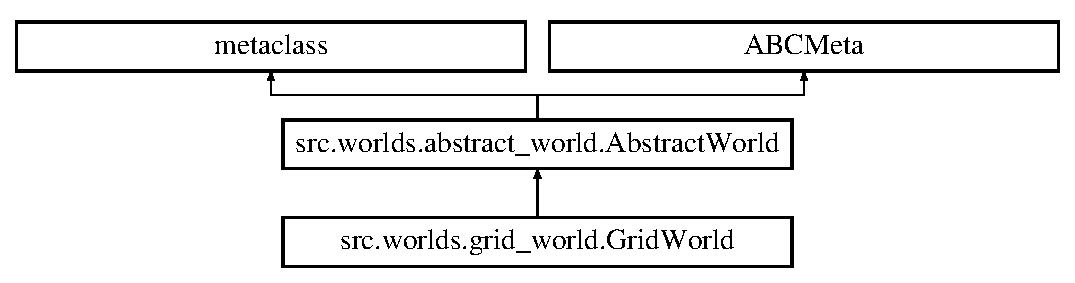
\includegraphics[height=3.000000cm]{classsrc_1_1worlds_1_1abstract__world_1_1_abstract_world}
\end{center}
\end{figure}
\subsection*{Public Member Functions}
\begin{DoxyCompactItemize}
\item 
\mbox{\Hypertarget{classsrc_1_1worlds_1_1abstract__world_1_1_abstract_world_a8bdd47c57f049a3e396ea64f4659db77}\label{classsrc_1_1worlds_1_1abstract__world_1_1_abstract_world_a8bdd47c57f049a3e396ea64f4659db77}} 
def {\bfseries \+\_\+\+\_\+init\+\_\+\+\_\+} (self)
\item 
\mbox{\Hypertarget{classsrc_1_1worlds_1_1abstract__world_1_1_abstract_world_a9da9b2c6a2403e83b08ba43d53a43d7d}\label{classsrc_1_1worlds_1_1abstract__world_1_1_abstract_world_a9da9b2c6a2403e83b08ba43d53a43d7d}} 
def {\bfseries states} (self)
\item 
\mbox{\Hypertarget{classsrc_1_1worlds_1_1abstract__world_1_1_abstract_world_a341fa28f1e3f825d1a26f4b23c438fb9}\label{classsrc_1_1worlds_1_1abstract__world_1_1_abstract_world_a341fa28f1e3f825d1a26f4b23c438fb9}} 
def {\bfseries state\+\_\+actions} (self, state)
\item 
\mbox{\Hypertarget{classsrc_1_1worlds_1_1abstract__world_1_1_abstract_world_adbb238f1675445eab7c0b002f9860aec}\label{classsrc_1_1worlds_1_1abstract__world_1_1_abstract_world_adbb238f1675445eab7c0b002f9860aec}} 
def {\bfseries transitions} (self, state, action)
\item 
\mbox{\Hypertarget{classsrc_1_1worlds_1_1abstract__world_1_1_abstract_world_a79b8c2b7f122d0d2463736248417dcec}\label{classsrc_1_1worlds_1_1abstract__world_1_1_abstract_world_a79b8c2b7f122d0d2463736248417dcec}} 
def {\bfseries run\+\_\+policy} (self, policy, iterations=1)
\item 
\mbox{\Hypertarget{classsrc_1_1worlds_1_1abstract__world_1_1_abstract_world_a3ef3e0539760634d7edfb132ee994cbb}\label{classsrc_1_1worlds_1_1abstract__world_1_1_abstract_world_a3ef3e0539760634d7edfb132ee994cbb}} 
def {\bfseries perform\+\_\+action} (self, state, action)
\item 
\mbox{\Hypertarget{classsrc_1_1worlds_1_1abstract__world_1_1_abstract_world_a1c5c774e258d31c703dc7a95280a686d}\label{classsrc_1_1worlds_1_1abstract__world_1_1_abstract_world_a1c5c774e258d31c703dc7a95280a686d}} 
def \hyperlink{classsrc_1_1worlds_1_1abstract__world_1_1_abstract_world_a1c5c774e258d31c703dc7a95280a686d}{get\+\_\+states} (self)
\begin{DoxyCompactList}\small\item\em Returns a list of all available states. \end{DoxyCompactList}\item 
def \hyperlink{classsrc_1_1worlds_1_1abstract__world_1_1_abstract_world_a177196a17a32460d8076eaffa643646b}{get\+\_\+actions} (self, state)
\begin{DoxyCompactList}\small\item\em Returns a list of all actions for a given state. \end{DoxyCompactList}\end{DoxyCompactItemize}


\subsection{Detailed Description}
Abstract Class for all worlds. 

\subsection{Member Function Documentation}
\mbox{\Hypertarget{classsrc_1_1worlds_1_1abstract__world_1_1_abstract_world_a177196a17a32460d8076eaffa643646b}\label{classsrc_1_1worlds_1_1abstract__world_1_1_abstract_world_a177196a17a32460d8076eaffa643646b}} 
\index{src\+::worlds\+::abstract\+\_\+world\+::\+Abstract\+World@{src\+::worlds\+::abstract\+\_\+world\+::\+Abstract\+World}!get\+\_\+actions@{get\+\_\+actions}}
\index{get\+\_\+actions@{get\+\_\+actions}!src\+::worlds\+::abstract\+\_\+world\+::\+Abstract\+World@{src\+::worlds\+::abstract\+\_\+world\+::\+Abstract\+World}}
\subsubsection{\texorpdfstring{get\+\_\+actions()}{get\_actions()}}
{\footnotesize\ttfamily def src.\+worlds.\+abstract\+\_\+world.\+Abstract\+World.\+get\+\_\+actions (\begin{DoxyParamCaption}\item[{}]{self,  }\item[{}]{state }\end{DoxyParamCaption})}



Returns a list of all actions for a given state. 


\begin{DoxyParams}{Parameters}
{\em state} & the state @\+:return actions \\
\hline
\end{DoxyParams}


The documentation for this class was generated from the following file\+:\begin{DoxyCompactItemize}
\item 
src/worlds/abstract\+\_\+world.\+py\end{DoxyCompactItemize}

\hypertarget{classsrc_1_1agent_1_1_agent}{}\section{src.\+agent.\+Agent Class Reference}
\label{classsrc_1_1agent_1_1_agent}\index{src.\+agent.\+Agent@{src.\+agent.\+Agent}}


Our agent class.  


\subsection*{Public Member Functions}
\begin{DoxyCompactItemize}
\item 
def \hyperlink{classsrc_1_1agent_1_1_agent_a86883ad8e273a62d61634e0ecbdcf1ed}{\+\_\+\+\_\+init\+\_\+\+\_\+} (self, keyword\+\_\+parameters)
\begin{DoxyCompactList}\small\item\em Constructor. \end{DoxyCompactList}\item 
\mbox{\Hypertarget{classsrc_1_1agent_1_1_agent_a40e0b7be81cba0248f4b6273d357eb27}\label{classsrc_1_1agent_1_1_agent_a40e0b7be81cba0248f4b6273d357eb27}} 
def \hyperlink{classsrc_1_1agent_1_1_agent_a40e0b7be81cba0248f4b6273d357eb27}{set\+\_\+policy} (self, policy\+\_\+)
\begin{DoxyCompactList}\small\item\em Mutator\+: Sets policy attribute. \end{DoxyCompactList}\item 
def \hyperlink{classsrc_1_1agent_1_1_agent_a5c84bc253f7ae188d87a839dbe73773a}{set\+\_\+world} (self, world\+\_\+)
\begin{DoxyCompactList}\small\item\em Mutator\+: Set world attribute. \end{DoxyCompactList}\item 
\mbox{\Hypertarget{classsrc_1_1agent_1_1_agent_af8dd43908b13ad19e99141f606a9beab}\label{classsrc_1_1agent_1_1_agent_af8dd43908b13ad19e99141f606a9beab}} 
def \hyperlink{classsrc_1_1agent_1_1_agent_af8dd43908b13ad19e99141f606a9beab}{generate\+\_\+policy} (self, world)
\begin{DoxyCompactList}\small\item\em Generates a new policy for the set world using the set policy\+Algorithm. \end{DoxyCompactList}\end{DoxyCompactItemize}
\subsection*{Public Attributes}
\begin{DoxyCompactItemize}
\item 
\mbox{\Hypertarget{classsrc_1_1agent_1_1_agent_aca24ae6676dedefced214e91ab59f00e}\label{classsrc_1_1agent_1_1_agent_aca24ae6676dedefced214e91ab59f00e}} 
{\bfseries policy\+\_\+algorithm}
\item 
\mbox{\Hypertarget{classsrc_1_1agent_1_1_agent_aa0cf3c2461ab9f02d74346aef220a9fb}\label{classsrc_1_1agent_1_1_agent_aa0cf3c2461ab9f02d74346aef220a9fb}} 
{\bfseries world}
\item 
\mbox{\Hypertarget{classsrc_1_1agent_1_1_agent_ad7643c30d167776e65804a2b7c8d66ef}\label{classsrc_1_1agent_1_1_agent_ad7643c30d167776e65804a2b7c8d66ef}} 
{\bfseries policy}
\end{DoxyCompactItemize}


\subsection{Detailed Description}
Our agent class. 



\subsection{Constructor \& Destructor Documentation}
\mbox{\Hypertarget{classsrc_1_1agent_1_1_agent_a86883ad8e273a62d61634e0ecbdcf1ed}\label{classsrc_1_1agent_1_1_agent_a86883ad8e273a62d61634e0ecbdcf1ed}} 
\index{src\+::agent\+::\+Agent@{src\+::agent\+::\+Agent}!\+\_\+\+\_\+init\+\_\+\+\_\+@{\+\_\+\+\_\+init\+\_\+\+\_\+}}
\index{\+\_\+\+\_\+init\+\_\+\+\_\+@{\+\_\+\+\_\+init\+\_\+\+\_\+}!src\+::agent\+::\+Agent@{src\+::agent\+::\+Agent}}
\subsubsection{\texorpdfstring{\+\_\+\+\_\+init\+\_\+\+\_\+()}{\_\_init\_\_()}}
{\footnotesize\ttfamily def src.\+agent.\+Agent.\+\_\+\+\_\+init\+\_\+\+\_\+ (\begin{DoxyParamCaption}\item[{}]{self,  }\item[{}]{keyword\+\_\+parameters }\end{DoxyParamCaption})}



Constructor. 


\begin{DoxyParams}{Parameters}
{\em a} & keyword dictionary with optional \\
\hline
\end{DoxyParams}


\subsection{Member Function Documentation}
\mbox{\Hypertarget{classsrc_1_1agent_1_1_agent_a5c84bc253f7ae188d87a839dbe73773a}\label{classsrc_1_1agent_1_1_agent_a5c84bc253f7ae188d87a839dbe73773a}} 
\index{src\+::agent\+::\+Agent@{src\+::agent\+::\+Agent}!set\+\_\+world@{set\+\_\+world}}
\index{set\+\_\+world@{set\+\_\+world}!src\+::agent\+::\+Agent@{src\+::agent\+::\+Agent}}
\subsubsection{\texorpdfstring{set\+\_\+world()}{set\_world()}}
{\footnotesize\ttfamily def src.\+agent.\+Agent.\+set\+\_\+world (\begin{DoxyParamCaption}\item[{}]{self,  }\item[{}]{world\+\_\+ }\end{DoxyParamCaption})}



Mutator\+: Set world attribute. 



The documentation for this class was generated from the following file\+:\begin{DoxyCompactItemize}
\item 
src/agent.\+py\end{DoxyCompactItemize}

\hypertarget{classsrc_1_1user__interface_1_1command__line__interface_1_1_command_line_interface}{}\section{src.\+user\+\_\+interface.\+command\+\_\+line\+\_\+interface.\+Command\+Line\+Interface Class Reference}
\label{classsrc_1_1user__interface_1_1command__line__interface_1_1_command_line_interface}\index{src.\+user\+\_\+interface.\+command\+\_\+line\+\_\+interface.\+Command\+Line\+Interface@{src.\+user\+\_\+interface.\+command\+\_\+line\+\_\+interface.\+Command\+Line\+Interface}}


Command Line User Interface.  


Inheritance diagram for src.\+user\+\_\+interface.\+command\+\_\+line\+\_\+interface.\+Command\+Line\+Interface\+:\begin{figure}[H]
\begin{center}
\leavevmode
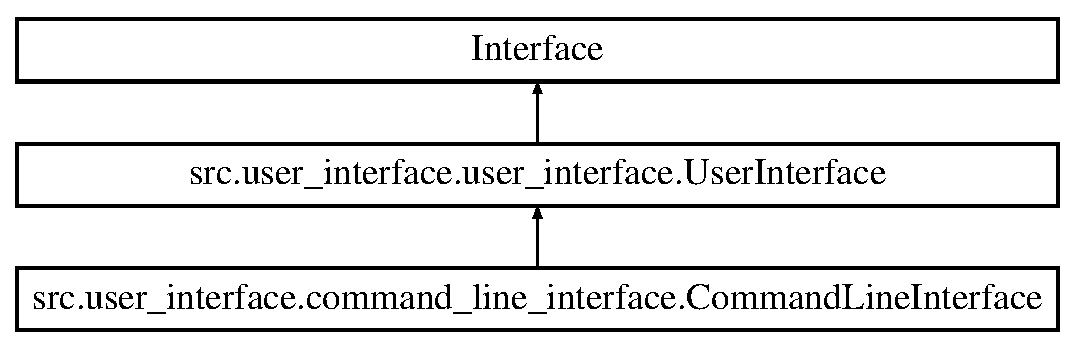
\includegraphics[height=3.000000cm]{classsrc_1_1user__interface_1_1command__line__interface_1_1_command_line_interface}
\end{center}
\end{figure}


\subsection{Detailed Description}
Command Line User Interface. 

The documentation for this class was generated from the following file\+:\begin{DoxyCompactItemize}
\item 
src/user\+\_\+interface/command\+\_\+line\+\_\+interface.\+py\end{DoxyCompactItemize}

\hypertarget{classsrc_1_1worlds_1_1grid__world_1_1_grid_world}{}\section{src.\+worlds.\+grid\+\_\+world.\+Grid\+World Class Reference}
\label{classsrc_1_1worlds_1_1grid__world_1_1_grid_world}\index{src.\+worlds.\+grid\+\_\+world.\+Grid\+World@{src.\+worlds.\+grid\+\_\+world.\+Grid\+World}}


Grid World.  


Inheritance diagram for src.\+worlds.\+grid\+\_\+world.\+Grid\+World\+:\begin{figure}[H]
\begin{center}
\leavevmode
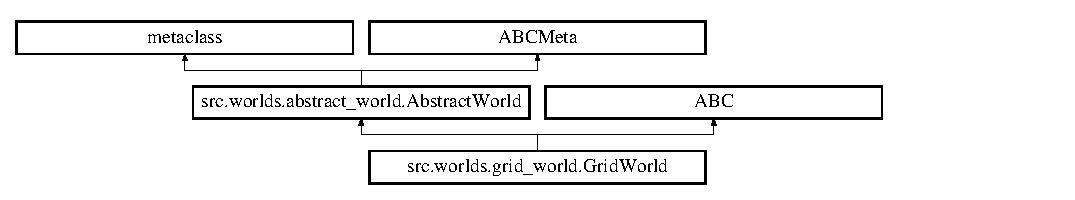
\includegraphics[height=2.240000cm]{classsrc_1_1worlds_1_1grid__world_1_1_grid_world}
\end{center}
\end{figure}
\subsection*{Public Member Functions}
\begin{DoxyCompactItemize}
\item 
\mbox{\Hypertarget{classsrc_1_1worlds_1_1grid__world_1_1_grid_world_afe3c1b392afbc00fb9a76c14a6e07899}\label{classsrc_1_1worlds_1_1grid__world_1_1_grid_world_afe3c1b392afbc00fb9a76c14a6e07899}} 
def {\bfseries \+\_\+\+\_\+init\+\_\+\+\_\+} (self)
\item 
\mbox{\Hypertarget{classsrc_1_1worlds_1_1grid__world_1_1_grid_world_a2ec82897b648609647d645f9b5835593}\label{classsrc_1_1worlds_1_1grid__world_1_1_grid_world_a2ec82897b648609647d645f9b5835593}} 
def {\bfseries run\+\_\+policy} (self, policy, iterations=1)
\item 
def \hyperlink{classsrc_1_1worlds_1_1grid__world_1_1_grid_world_a93de8a88475e8ad0530fe703343028c9}{perform\+\_\+action} (self, state, action)
\begin{DoxyCompactList}\small\item\em Determines the reward and resulting state after performing an action on the given state. \end{DoxyCompactList}\end{DoxyCompactItemize}


\subsection{Detailed Description}
Grid World. 

\subsection{Member Function Documentation}
\mbox{\Hypertarget{classsrc_1_1worlds_1_1grid__world_1_1_grid_world_a93de8a88475e8ad0530fe703343028c9}\label{classsrc_1_1worlds_1_1grid__world_1_1_grid_world_a93de8a88475e8ad0530fe703343028c9}} 
\index{src\+::worlds\+::grid\+\_\+world\+::\+Grid\+World@{src\+::worlds\+::grid\+\_\+world\+::\+Grid\+World}!perform\+\_\+action@{perform\+\_\+action}}
\index{perform\+\_\+action@{perform\+\_\+action}!src\+::worlds\+::grid\+\_\+world\+::\+Grid\+World@{src\+::worlds\+::grid\+\_\+world\+::\+Grid\+World}}
\subsubsection{\texorpdfstring{perform\+\_\+action()}{perform\_action()}}
{\footnotesize\ttfamily def src.\+worlds.\+grid\+\_\+world.\+Grid\+World.\+perform\+\_\+action (\begin{DoxyParamCaption}\item[{}]{self,  }\item[{}]{state,  }\item[{}]{action }\end{DoxyParamCaption})}



Determines the reward and resulting state after performing an action on the given state. 

Actions selected are weighted using the probabilities defined in self.\+\_\+state\+\_\+actions.\+get(state, action)


\begin{DoxyParams}{Parameters}
{\em state} & The starting state \\
\hline
{\em action} & The action to perform \\
\hline
\end{DoxyParams}
\begin{DoxyReturn}{Returns}
the resulting state, the reward 
\end{DoxyReturn}


The documentation for this class was generated from the following file\+:\begin{DoxyCompactItemize}
\item 
src/worlds/grid\+\_\+world.\+py\end{DoxyCompactItemize}

\hypertarget{classsrc_1_1user__interface_1_1gui__interface_1_1_g_u_i_interface}{}\section{src.\+user\+\_\+interface.\+gui\+\_\+interface.\+G\+U\+I\+Interface Class Reference}
\label{classsrc_1_1user__interface_1_1gui__interface_1_1_g_u_i_interface}\index{src.\+user\+\_\+interface.\+gui\+\_\+interface.\+G\+U\+I\+Interface@{src.\+user\+\_\+interface.\+gui\+\_\+interface.\+G\+U\+I\+Interface}}


G\+UI User Interface.  


Inheritance diagram for src.\+user\+\_\+interface.\+gui\+\_\+interface.\+G\+U\+I\+Interface\+:\begin{figure}[H]
\begin{center}
\leavevmode
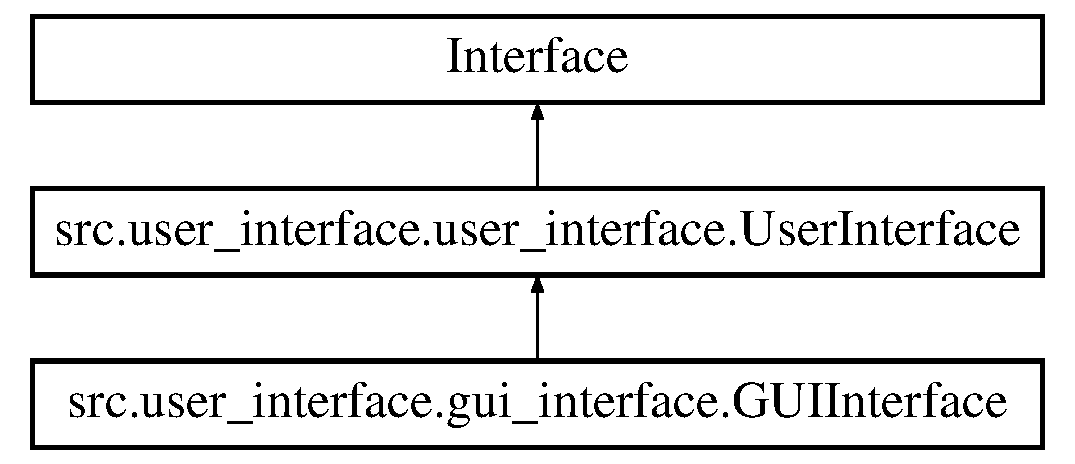
\includegraphics[height=3.000000cm]{classsrc_1_1user__interface_1_1gui__interface_1_1_g_u_i_interface}
\end{center}
\end{figure}


\subsection{Detailed Description}
G\+UI User Interface. 

The documentation for this class was generated from the following file\+:\begin{DoxyCompactItemize}
\item 
src/user\+\_\+interface/gui\+\_\+interface.\+py\end{DoxyCompactItemize}

\hypertarget{classsrc_1_1policy__algorithms_1_1policy__algorithm_1_1_policy_algorithm}{}\section{src.\+policy\+\_\+algorithms.\+policy\+\_\+algorithm.\+Policy\+Algorithm Class Reference}
\label{classsrc_1_1policy__algorithms_1_1policy__algorithm_1_1_policy_algorithm}\index{src.\+policy\+\_\+algorithms.\+policy\+\_\+algorithm.\+Policy\+Algorithm@{src.\+policy\+\_\+algorithms.\+policy\+\_\+algorithm.\+Policy\+Algorithm}}


Policy Algorithm Interface.  


Inheritance diagram for src.\+policy\+\_\+algorithms.\+policy\+\_\+algorithm.\+Policy\+Algorithm\+:\begin{figure}[H]
\begin{center}
\leavevmode
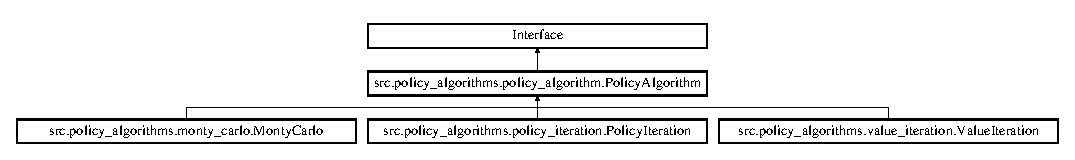
\includegraphics[height=1.707317cm]{classsrc_1_1policy__algorithms_1_1policy__algorithm_1_1_policy_algorithm}
\end{center}
\end{figure}
\subsection*{Public Member Functions}
\begin{DoxyCompactItemize}
\item 
\mbox{\Hypertarget{classsrc_1_1policy__algorithms_1_1policy__algorithm_1_1_policy_algorithm_a54e71e409c15ddf266dffceb4773e30b}\label{classsrc_1_1policy__algorithms_1_1policy__algorithm_1_1_policy_algorithm_a54e71e409c15ddf266dffceb4773e30b}} 
def {\bfseries generate\+\_\+policy} (self, world)
\end{DoxyCompactItemize}


\subsection{Detailed Description}
Policy Algorithm Interface. 

The documentation for this class was generated from the following file\+:\begin{DoxyCompactItemize}
\item 
src/policy\+\_\+algorithms/policy\+\_\+algorithm.\+py\end{DoxyCompactItemize}

\hypertarget{classsrc_1_1policy__algorithms_1_1policy__iteration_1_1_policy_iteration}{}\section{src.\+policy\+\_\+algorithms.\+policy\+\_\+iteration.\+Policy\+Iteration Class Reference}
\label{classsrc_1_1policy__algorithms_1_1policy__iteration_1_1_policy_iteration}\index{src.\+policy\+\_\+algorithms.\+policy\+\_\+iteration.\+Policy\+Iteration@{src.\+policy\+\_\+algorithms.\+policy\+\_\+iteration.\+Policy\+Iteration}}


Policy Iteration Algorithm.  


Inheritance diagram for src.\+policy\+\_\+algorithms.\+policy\+\_\+iteration.\+Policy\+Iteration\+:\begin{figure}[H]
\begin{center}
\leavevmode
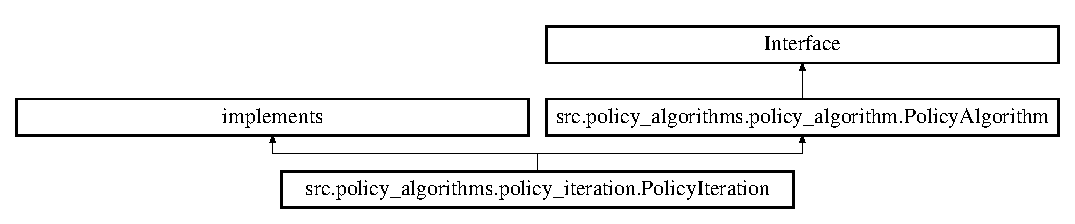
\includegraphics[height=2.560976cm]{classsrc_1_1policy__algorithms_1_1policy__iteration_1_1_policy_iteration}
\end{center}
\end{figure}
\subsection*{Public Member Functions}
\begin{DoxyCompactItemize}
\item 
\mbox{\Hypertarget{classsrc_1_1policy__algorithms_1_1policy__iteration_1_1_policy_iteration_a7ee703e2982604f37990128d183e5422}\label{classsrc_1_1policy__algorithms_1_1policy__iteration_1_1_policy_iteration_a7ee703e2982604f37990128d183e5422}} 
def {\bfseries generate\+\_\+policy} (self, world)
\end{DoxyCompactItemize}


\subsection{Detailed Description}
Policy Iteration Algorithm. 

Uses policy iteration to generate policies 

The documentation for this class was generated from the following file\+:\begin{DoxyCompactItemize}
\item 
src/policy\+\_\+algorithms/policy\+\_\+iteration.\+py\end{DoxyCompactItemize}

\hypertarget{classsrc_1_1user__interface_1_1user__interface_1_1_user_interface}{}\section{src.\+user\+\_\+interface.\+user\+\_\+interface.\+User\+Interface Class Reference}
\label{classsrc_1_1user__interface_1_1user__interface_1_1_user_interface}\index{src.\+user\+\_\+interface.\+user\+\_\+interface.\+User\+Interface@{src.\+user\+\_\+interface.\+user\+\_\+interface.\+User\+Interface}}


General Interface for all user interfaces.  


Inheritance diagram for src.\+user\+\_\+interface.\+user\+\_\+interface.\+User\+Interface\+:\begin{figure}[H]
\begin{center}
\leavevmode
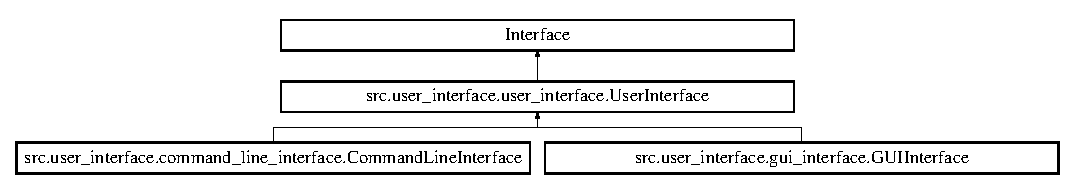
\includegraphics[height=2.110553cm]{classsrc_1_1user__interface_1_1user__interface_1_1_user_interface}
\end{center}
\end{figure}


\subsection{Detailed Description}
General Interface for all user interfaces. 

The documentation for this class was generated from the following file\+:\begin{DoxyCompactItemize}
\item 
src/user\+\_\+interface/user\+\_\+interface.\+py\end{DoxyCompactItemize}

\hypertarget{classsrc_1_1policy__algorithms_1_1value__iteration_1_1_value_iteration}{}\section{src.\+policy\+\_\+algorithms.\+value\+\_\+iteration.\+Value\+Iteration Class Reference}
\label{classsrc_1_1policy__algorithms_1_1value__iteration_1_1_value_iteration}\index{src.\+policy\+\_\+algorithms.\+value\+\_\+iteration.\+Value\+Iteration@{src.\+policy\+\_\+algorithms.\+value\+\_\+iteration.\+Value\+Iteration}}


Value Iteration Algorithm.  


Inheritance diagram for src.\+policy\+\_\+algorithms.\+value\+\_\+iteration.\+Value\+Iteration\+:\begin{figure}[H]
\begin{center}
\leavevmode
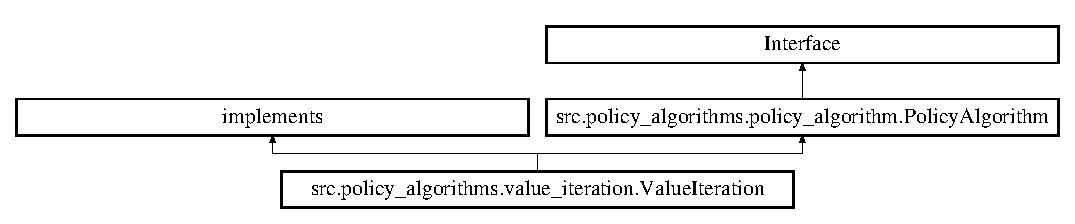
\includegraphics[height=2.560976cm]{classsrc_1_1policy__algorithms_1_1value__iteration_1_1_value_iteration}
\end{center}
\end{figure}
\subsection*{Public Member Functions}
\begin{DoxyCompactItemize}
\item 
\mbox{\Hypertarget{classsrc_1_1policy__algorithms_1_1value__iteration_1_1_value_iteration_a4d494ddb4ea4ce78858f5ee0b113a401}\label{classsrc_1_1policy__algorithms_1_1value__iteration_1_1_value_iteration_a4d494ddb4ea4ce78858f5ee0b113a401}} 
def {\bfseries generate\+\_\+policy} (self, world)
\end{DoxyCompactItemize}


\subsection{Detailed Description}
Value Iteration Algorithm. 

Uses value iteration to generate policies 

The documentation for this class was generated from the following file\+:\begin{DoxyCompactItemize}
\item 
src/policy\+\_\+algorithms/value\+\_\+iteration.\+py\end{DoxyCompactItemize}

%--- End generated contents ---

% Index
\backmatter
\newpage
\phantomsection
\clearemptydoublepage
\addcontentsline{toc}{chapter}{Index}
\printindex

\end{document}
